% paper_zh.tex — 中文版 preprint 源文件，生成于 2026-10-14，译自 04_manuscript_zh.md
%（《拟合实践，而非作品：一种以人为参照的 AGI 理论》，
%   英文版 04_manuscript.md / paper.tex）。
% 编译：`tectonic paper_zh.tex`（自动运行 BibTeX 生成 paper_zh.bbl；需要
%        references.bib + figures/ 在同目录）。若自动 BibTeX 未运行，
%        可复制 paper.bbl 为 paper_zh.bbl。
% XeLaTeX + ctexart：不要加 fontenc/inputenc/newtx（与 CJK 冲突）。
% 图为英文原图，原样复用；图注中引用图上文字处保留英文。

\documentclass[10pt,fontset=fandol]{ctexart}
\usepackage{amsmath}
\usepackage{amssymb}

\usepackage[margin=1in]{geometry}
\setlength{\emergencystretch}{2em}
\usepackage{graphicx}
\graphicspath{{figures/}}
\usepackage{booktabs}
\usepackage{array}
\usepackage[numbers,sort&compress]{natbib}
\usepackage{xcolor}
\usepackage[colorlinks=true,linkcolor=blue!60!black,citecolor=blue!60!black,urlcolor=blue!60!black]{hyperref}
\urlstyle{same}

% 带圈数字 ①-⑳（U+2460–2473）按 CJK 处理，走中文字体（拉丁字体无此字形）
\xeCJKDeclareCharClass{CJK}{"2460 -> "2473}

\newcommand{\dminus}{-}

\title{\textbf{拟合实践，而非作品：\\一种以人为参照的 AGI 理论}}

\author{余玉桂\\
余玉桂战略研究室\\
\texttt{they4897@gmail.com}
}

\date{2026 年 10 月 19 日修订（初版 2026 年 10 月 15 日）}

\begin{document}
\maketitle

\begin{abstract}
\noindent 本文提出一种以人为参照（human-referential）的人工通用智能（AGI）理论，包含三个相互关联的论断。在概念层面，AGI 是一个哲学概念：只要“通用性”以人类实践的开放集合为参照，它就无法被还原为一份技术规格。在实现层面，AGI 的手段是对人类实践的拟合——而不是对人类积累作品的拟合。在规范层面，AGI 应被定位为增强性工具（augmentative tool），而非新主体。理论的核心是一条时间性条款（temporal clause）：\textbf{拟合对象不是人类的作品，而是人类的实践——人类经验的全谱（横截面）与全程（纵截面）。存量有墙，流量无墙。}为使该理论可审计而非仅具纲领性，我们构建了一幅结构化证据地图（evidence map）：一个目的性抽样的 $N = 80$ 作品语料，在两条立场轴（描述性与规范性）与八个拟合对象维度上编码。地图量化了理论的核心缺口：经验类型轴（成功/失败、专家/新手、典型/边缘）在 0/80 篇作品中被显式处理（精确二项 95\% CI $[0.0\%, 4.5\%]$），实践即流量仅在 2/80 篇作品中显式出现，且均来自 2026 年；作品即存量自 2022 年起获得连续的显式处理，输出分布覆盖则首次出现于 2024 年。我们导出理论在分布、生产与治理上的三点方法论蕴含，并陈述证伪条件。
\end{abstract}

\medskip
\noindent\textbf{关键词：} 人工通用智能；实践拟合；以人为参照的拟合；数据墙；增强；证据地图

\section{引言}\label{sec:intro}

拆开来看，每一个前沿模型都是对人类产出之物的蒸馏——网络文本、代码、数学、评分。“在人类数据上训练”这句话熟悉到其歧义无人察觉。它容许两种解读，而两者分岔为不同的研究纲领。在静态解读下，拟合对象是人类的作品：一个有限的、已被产出的档案，可被爬取、清洗、去重、穷尽。在动态解读下，拟合对象是人类的实践：经验的持续再生——工具使用、交互、反馈、失败、修复——只要生命延续，它就延续。我们称前者为语料拟合（corpus-fitting），后者为实践拟合（practice-fitting）。当前静态解读占主导：扩展性分析以公共人类生成文本的有限存量为推理对象（估计约 300 万亿 token \cite{villalobos2022data}）；旗舰技术报告记录档案语料之上的静态配比 \cite{grattafiori2024llama3}。本文辩护的是动态解读。

这一区分由一句话固定，我们称之为时间性条款，它防止理论最常见的误读：

\begin{quote}
\textbf{拟合对象不是人类的作品，而是人类的实践——人类经验的全谱（横截面）与全程（纵截面）。存量有墙，流量无墙。}
\end{quote}

两条轴构成拟合目标。全谱（full spectrum）是横截面轴：谁被代表，以及哪些种类的经验——成功与失败、专家与新手、典型与边缘。全程（full course）是纵截面轴：实践的时间流，任何快照都无法存档。存量/流量不对称在本理论中有精确含义：数据墙 \cite{villalobos2022data} 是存量的属性，而非人类学极限；在生成数据上递归训练导致的模型坍塌 \cite{shumailov2024collapse}，是把存量当作可自我更新之物来对待的病理。流量侧数据——生产遥测、交互日志、失败提交——随部署而再生。这一区分的哲学骨架是阿伦特对劳动、制作与行动的三分 \cite{arendt1958human}：静态误读只拟合制作的产物，而本理论以持续进行中的劳动与行动过程为拟合对象。

本文建立在此前一项实证审计 \cite{yu2026failure} 之上——该审计考察了行业在模型训练生命周期中如何处理失败数据，并记录其系统性弃置。那项审计测量的是存量丢弃了什么；本篇陈述理论——训练对象是实践而非作品，即从存量到流量的转向。流量如何采集、清洗并吸收，留待未来工作。

\paragraph{缺口。}
四类文献各自成熟却互不连通。文化技术分析告诉我们大模型\emph{是什么}——继承人类符号生产结构的技术 \cite{farrell2025cultural}。批判现象学告诉我们模型\emph{反射什么}——一面塑造人类自我理解的扭曲之镜 \cite{vallor2024mirror}。增强经济学告诉我们 AI \emph{应当是什么}——人类能动性的互补品而非替代品 \cite{brynjolfsson2022turing}。多元对齐告诉我们\emph{谁的价值}应当被拟合 \cite{gabriel2020values}。缺失的是把它们统一起来的连接命题——以拟合人类实践为手段、以增强人类为目的——连同数据方法论争论所缺少的时间性概念工具（存量与流量之别）。与此同时，一门计量学文献警告：我们的基准是人类实践的抽样投影，且常常是糟糕的投影 \cite{salaudeen2025measurement}，这使参照系问题无法回避，而不止是修辞。

\paragraph{术语防护。}
拟合（fitting）在此取其统计学含义（逼近一个分布或函数结构），并扩展至一个总体对象：人类生活形式的可表达投影。它比模仿（行为匹配）更宽，比对齐（一种规范关系）更窄。与拟态不同，拟合不预设“冒充人类”这一目标。事实上，本理论将论证：拟合作为手段可行，作为目的必败。

\paragraph{贡献。}
本文做出四项贡献：
\begin{enumerate}
\item \textbf{一个时间性区分}：拟合人类作品与拟合人类实践之分，以时间性条款的形式陈述，并配有命名术语（语料拟合与实践拟合之分；全谱 $\times$ 全程；拟合时差 fitting lag——日常实践再生与周期性模型快照之间的落差）。
\item \textbf{一个坐标系}：拟合目标的全谱 $\times$ 全程平面，识别出经验类型是当前实践所缺失的覆盖轴——在既有的两条轴（人群“谁”与输出分布）之外。
\item \textbf{一幅结构化证据地图}：承继配套审计论文编码手册精神的方法论组件 \cite{yu2026failure}，把理论的核心缺口变成可计数、可证伪的结果：经验类型轴在 80 篇作品中的显式处理为 0。
\item \textbf{四条终止边界}：流量侧拟合的终止条件（实践主体的终结；拟合者越界；制度边界；自指性污染），它们把时间性条款从口号变为有界断言。
\end{enumerate}

\paragraph{路线图。}
第~\ref{sec:concept} 节论证 AGI 是哲学概念。第~\ref{sec:implementation} 节展开实践拟合作为实现论题，正面处理三路反对，末尾以一节形式化概览（第~\ref{sec:formalsketch} 节）把存量/流量之别表述为一对优化问题，并把四条边界表述为停止条件。第~\ref{sec:position} 节陈述增强性工具立场，作为一种具有学术谱系的规范立场。第~\ref{sec:evidencemap} 节呈现证据地图：方法、表格、图与量化缺口。第~\ref{sec:tensions} 节处理张力并划定四条边界。第~\ref{sec:implications} 节导出三个面向未来工作的方法论蕴含。第~\ref{sec:conclusion} 节作结。

\section{概念：AGI 作为哲学概念}\label{sec:concept}

理论的第一项论断是概念性的：AGI 不是一份等待完成的工程规格，而是一个以人类实践为参照系的哲学概念。三股文献在此汇合。

\paragraph{定义谱系本身就是哲学的。}
Legg 与 Hutter 把普遍智能定义为在广泛环境范围内的目标达成——通用性由环境范围来衡量 \cite{legg2007universal}。Levels-of-AGI 框架把通用性 $\times$ 自主性操作化为层级分类 \cite{morris2023levels}。METR 任务时长基准测量 AI 能完成任务的时间视界：全序列的翻倍期估计约为七个月 \cite{kwa2025measuring}，其 2026 年更新把 2023--2026 段修订至约四个月 \cite{metr2026th11}——该更新的维护者自己标明任务套件已临天花板饱和，而已发表的批评进一步论证它不足以支撑强结论，理由包括任务套件的污染风险与人类基线来源的窄化 \cite{witkin2026metr}。我们因此把时间视界当作下述诸多操作化中的一个易错代理，而非实际承重的前提。这些操作化是有用的，但每一个都从对环境的隐式抽样中继承其“通用”概念——而对 AI 系统而言，环境是人类建造的使用情境。这些操作化是它们并未定义之概念的代理物。

\paragraph{计量学批判在这一点上是决定性的。}
一个以效度为中心的 AI 评估框架从心理测量学引入构念效度，发现大多数基准无法支撑建立于其上的断言 \cite{salaudeen2025measurement}。心理测量学传统的平行工作表明，语言模型中表面上的类认知能力对题目间相关性与测量设计敏感 \cite{ilic2024evidence}，而心理测量学导出的短基准会改变同一批模型的排序 \cite{gignac2025psychometrically}。共同推论是：基准任务是人类实践的抽样投影——一个基准只相对于它抽样的那一片实践才是通用的。一个其操作化是实践样本的概念，不可能脱离它所抽样的实践而漂浮。

\paragraph{移动靶批判从另一侧汇合。}
Tesler 定理——智能就是机器尚未做到之事——刻画了自 AI 创立以来伴随始终的定义的不断后退 \cite{tesler1997effect}；一篇新近文章把 AGI 与永动机的类比推向极致，称其为范畴错误而非硬目标 \cite{imeri2025benefits}；一项以严谨为导向的分析论证，AI 进步话语系统性地缺乏成熟科学的推理纪律 \cite{nguyen2026rigor}。倘若 AGI 是一个固定的技术目标，这些病理本可用更好的测量治愈。在本文辩护的观点下，它们反映的是这一概念的真实结构：只要“通用”以人类实践的开放集合为参照，AGI 就不可能是规格级的，因为参照集开放且移动——不是因为智能神秘。

\paragraph{哲学人类学提供正面理论支点。}
普莱斯纳的自然人工性法则认为，人在构成性意义上是人工的——一个通过人工物完成自身的有机体，以离心姿态定位于自身自然之外 \cite{plessner1928levels}。在这一人类学上，工具使用不是人性的断裂而是其常态；媒介技术时代对普莱斯纳的解读恰好把这一点延伸到数字人工物 \cite{demul2014philosophical}，而“翻译人”（Homo Translator）对仿生技术中人在回路的分析使“人—人工物”回路显豁 \cite{tamborini2025homo}。因此第~\ref{sec:position} 节辩护的工具立场无须为“仅仅是工具性”道歉：工具性是人类学常量，不是形而上学的降格。与吹捧和焦虑两种态度相比，普莱斯纳额外贡献的是一个判据：问题不在于人类是否用人工物完成自身（从来如此），而在于这个人工物是否被拟合到人类所做之事的全部范围——包括人类如何犯错。

图~\ref{fig:framework} 在这一坐标系中概括了理论：拟合对象从作品（静态存量，受墙约束）延伸到实践（再生流量）；纵轴是实践的全程；流量区域内标有既有的两条覆盖轴，并另行标出缺失的第三条；四条边界终止拟合。

\begin{figure}[t]
\centering
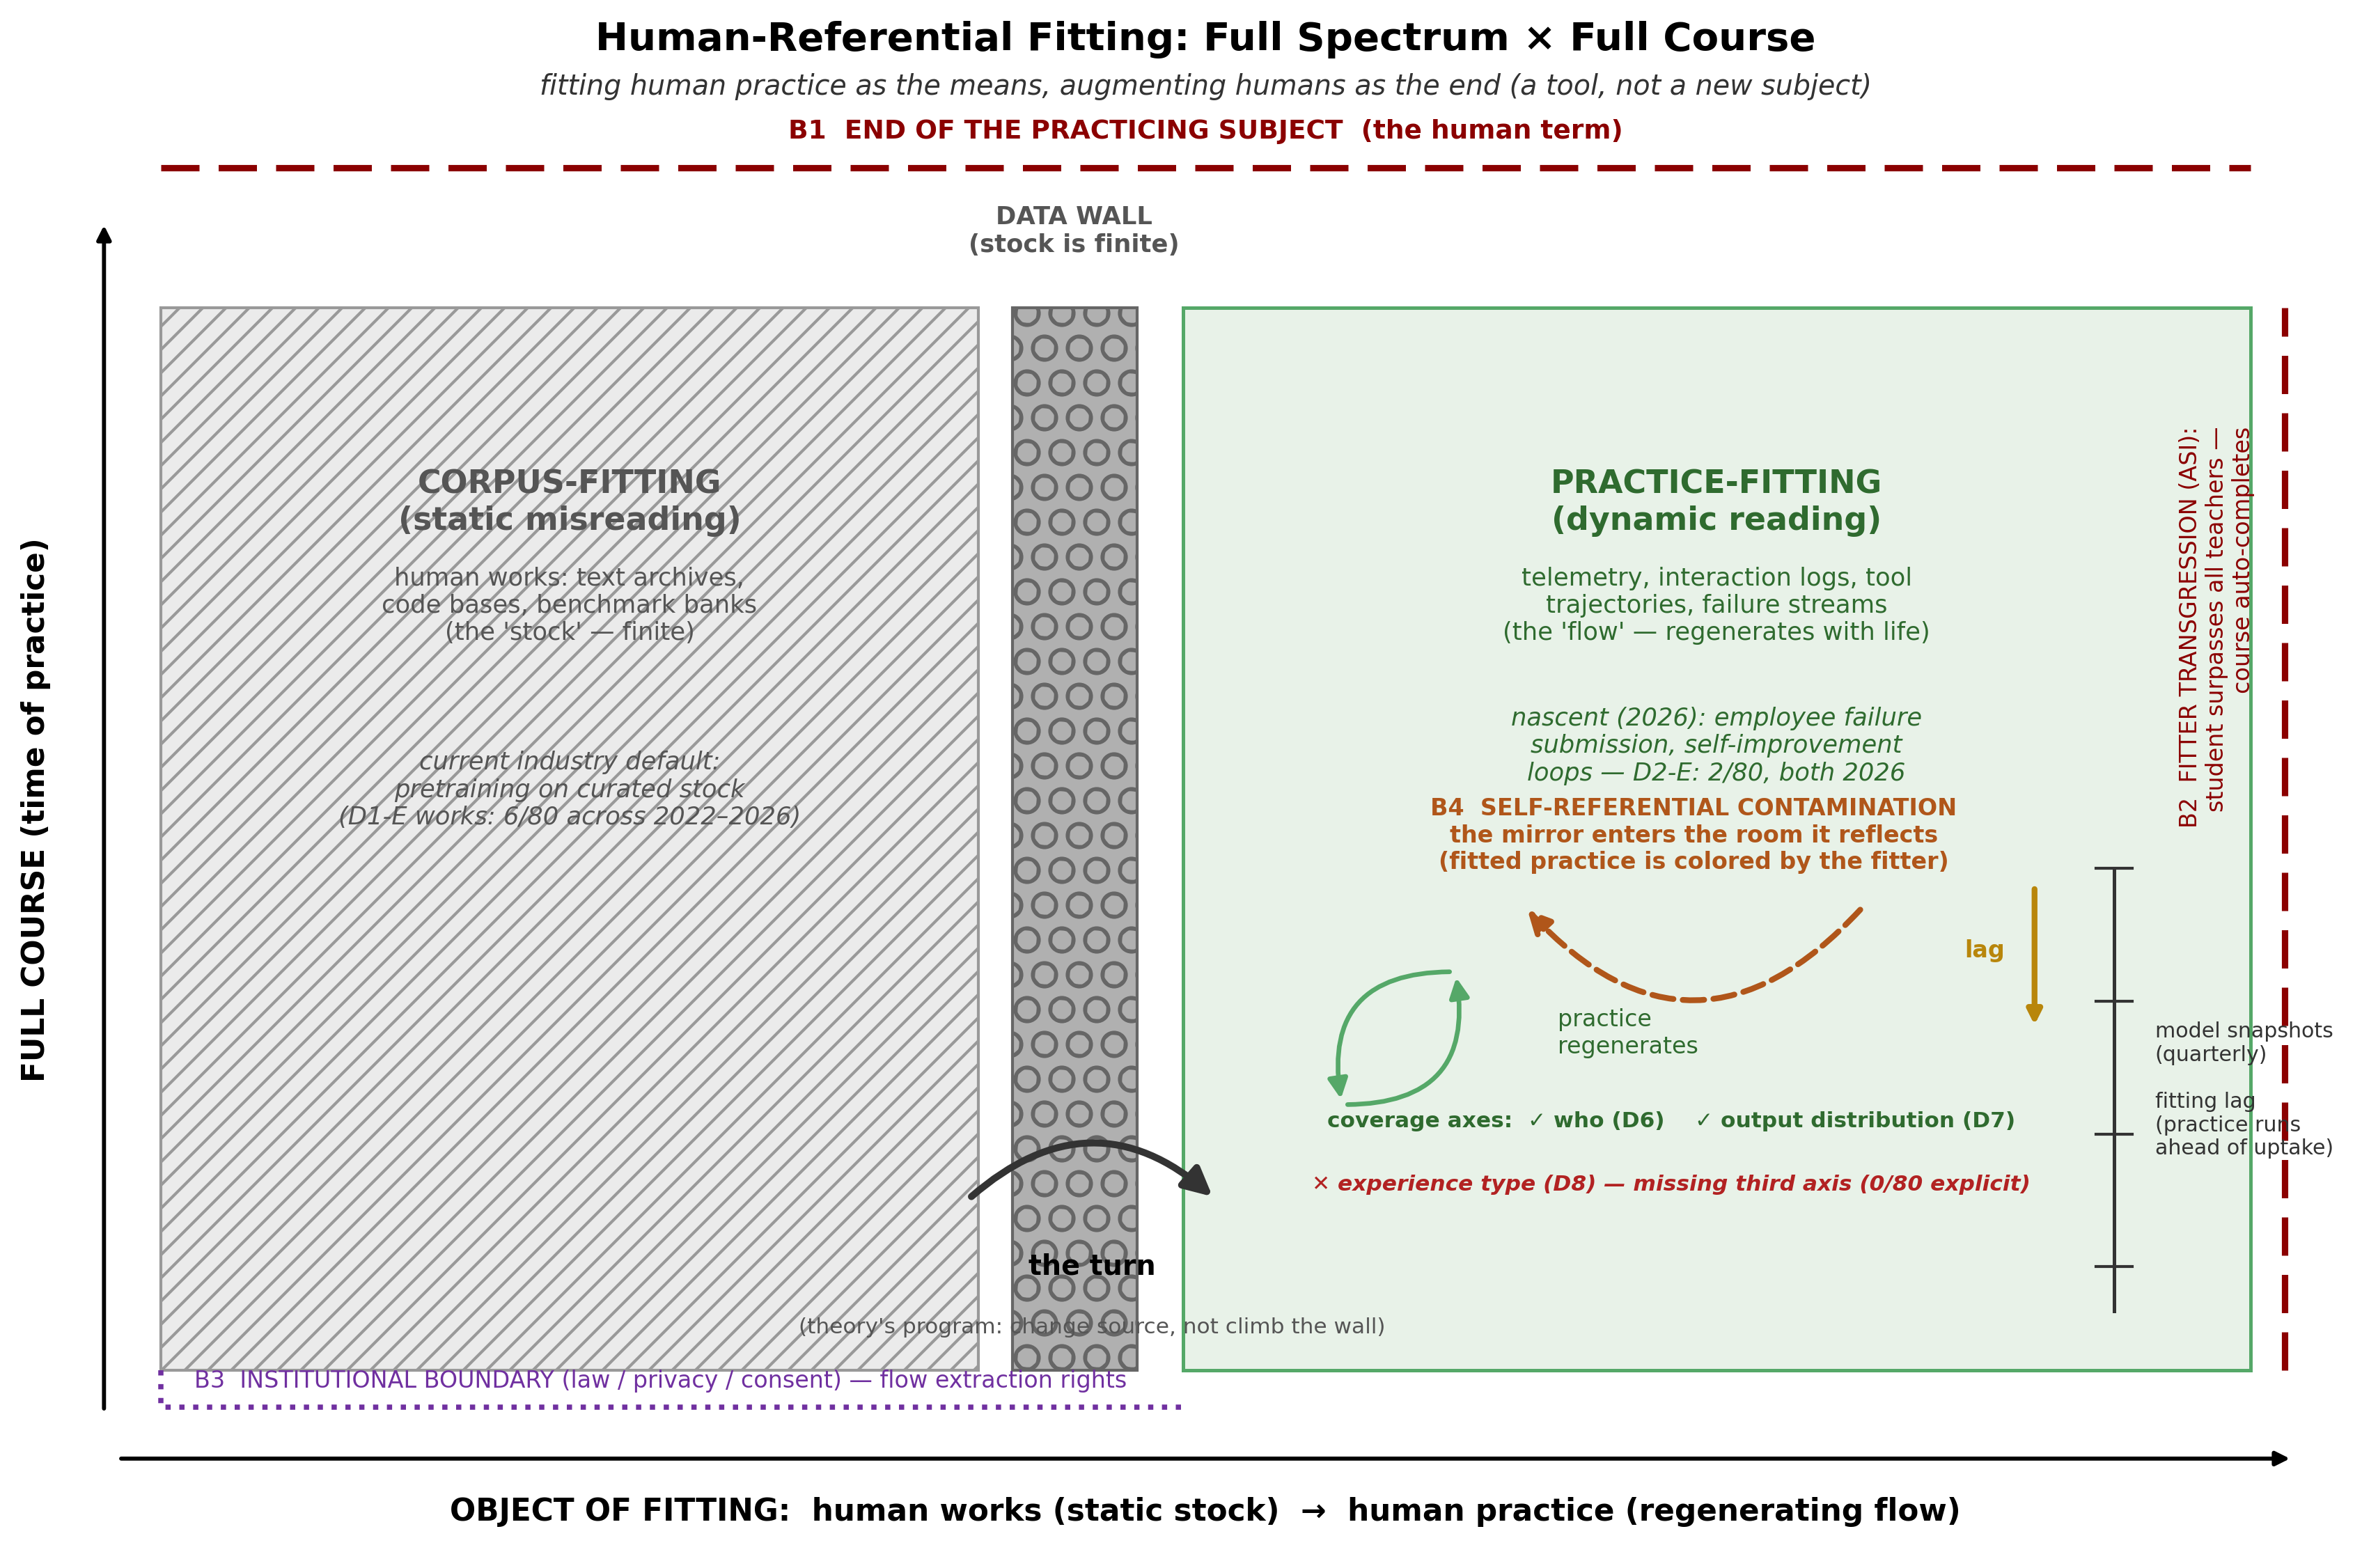
\includegraphics[width=\textwidth]{fig1_theory_framework.png}
\caption{理论一览：全谱 $\times$ 全程坐标系。横轴：拟合对象，从人类的作品（静态存量；砖纹 = 数据墙）到人类的实践（再生流量；环形箭头）。纵轴：实践的时间历程。流量区域内标注既有的两条覆盖轴（人群“谁”，D6；输出分布，D7）与缺失的第三轴（经验类型，D8；我们的语料中 0/80 篇作品）。右缘：拟合时差时间线——实践持续再生而模型快照周期性更新。四条终止边界被标出：B1，实践主体的终结（顶部，虚线）；B2，拟合者越界（右侧；拟合关系自行耗尽——不再存在尚未被它超越的人类实践）；B3，制度边界（底部，点线；法律、隐私、知情同意）；B4，自指性污染（回环弧线；“the mirror enters the room it reflects”）。中央“转向”箭头越过\emph{墙外}——改变源头而非翻越它。副标题：拟合为手段，增强为目的（是工具，不是新主体）。}
\label{fig:framework}
\end{figure}

三股之汇给出第一项论断。定义谱系无法闭合概念；测量批判表明操作化是实践样本；移动靶批判解释了原因；哲学人类学挡住了从“不可规格化”到“敌视技术”的推论。AGI 作为以人为参照的概念是透镜，不是倒计时。

\section{实现：实践拟合作为手段}\label{sec:implementation}

第二项论断关乎实现：通往 AGI 之路经过对人类实践的拟合——其知识、规范、功能性情绪—动机结构与失败模式——而这一拟合是\emph{手段}，不是目的。

\paragraph{文化技术论题设定框架。}
Farrell、Gopnik、Shalizi 与 Evans 在《科学》上论证，大型 AI 模型是文化与社会技术：像文字与市场一样，它们继承、传递并重组人类符号生产的结构，连同这种传递所伴生的病理 \cite{farrell2025cultural}。认知路线佐证：儿童经由模仿的文化学习表现出“传承与求真”的权衡，当前模型对此的处理方式不同 \cite{yiu2024transmission}；大模型仅从文本便自发发展出类人的类比推理 \cite{webb2023emergent}。如果模型是文化技术，其能力继承自人类实践——这使继承的\emph{质量}（传递什么、来自谁、包括错误）成为核心工程变量，而非事后注脚。

\paragraph{经验链条不再是思辨。}
GPT-4o 复现了由自由选择调节的类人认知失调与自我辩护模式 \cite{lehr2025kernels}；生成模型表现出类人社会身份偏差 \cite{hu2025generative}；可解释性工作已在生产模型内部识别出因果有效的情绪概念，影响其输出及其对自身角色的理解 \cite{anthropic2026emotions}。在价值侧，合作逆强化学习把 AI—人关系形式化为对未知人类奖励函数的协助 \cite{hadfield2016cooperative}；偏好学习训练出的奖励模型，在结构上就是人类偏好分布的拟合器 \cite{christiano2017deep, ouyang2022training}；近期工作明确论证：对齐的模型因而是关于人的模型 \cite{yuan2026aligned}。认知科学提供时间性注脚：描述—经验鸿沟表明，人类认知本身在从描述学习与从直接经验学习时并不相同 \cite{hertwig2009description}。预训练拟合的是对实践的描述；智能体化部署拟合的是实践本身——会再生的经验。

\paragraph{哲学基础。}
维特根斯坦的生活形式——语言在其中获得意义的、交织的实践模式 \cite{wittgenstein1953philosophical}——把拟合对象锚定于实践而非文本：关于分布学习是否足以产生意义的向量奠基之争，恰恰是关于文本投影保留了多少生活形式之争 \cite{mollo2026vector, mallory2023wittgenstein}，其中意义怀疑论与辩护立场双方都预设基准是人类用法 \cite{sogaard2023grounding}。上引阿伦特的三分提供时间骨架 \cite{arendt1958human}：静态误读拟合的是制作的沉积物；本理论拟合的是持续进行的劳动与行动。

\paragraph{精确化。}
拟合对象是人类生活形式的可表达投影——不是生物学的人。这同时挡住两种误读：理论不主张模型复制人格，也不主张拟合目标受限于已被写下之物。两个推论随之而来。其一，拟合人类的\emph{失败}与多样性是矫正方向：配套审计论文的审计表明行业弃置了经验中失败的那一半 \cite{yu2026failure}；理论解释了为何该弃置是覆盖错误而非数据卫生的成功。其二，拟合对象包括功能性情绪—动机结构 \cite{lehr2025kernels, hu2025generative, anthropic2026emotions}——但仅在功能层，这一边界第~\ref{sec:tensions} 节将予以划定。

\paragraph{三路反对必须正面应对。}

\emph{其一，蜂群证据。} 一项覆盖 70+ 模型的开放式生成大规模研究——基于 Infinity-Chat、获 NeurIPS 2025 荣誉——发现了显著的模式坍塌：无论解码配置如何，模型内重复与模型间同质化 \cite{jiang2025hivemind}。这是支持而非反驳本理论的证据：70+ 模型收敛到共享的类人分布，确认了拟合在发生；坍塌反驳的是对均值拟合的充分性。当语料既是所有人又不是任何人时，语料拟合出来的样子就是蜂群——它拟合的是均值，而非谱（“it fits the mean, not the spectrum”）。补救不是更少拟合而是更宽拟合：谱轴就是矫正。

\emph{其二，天花板论证。} 数据墙约束人类生成的公共文本存量 \cite{villalobos2022data}；在生成数据上的递归训练使模型退化 \cite{shumailov2024collapse}。两者皆真，且两者都是关于存量的断言——而两项新结果迫使我们把“墙”说得更准。对固定语料的对抗性自博弈——一个模型从存档文档中挖题、另一个解题、第三个裁判 \cite{liu2025spice}——以及把固定网络语料拉伸至约 1.8 倍数据效率的模型生成“兆档文档”（megadocs）\cite{kim2026megadocs}，表明档案几乎可以被无限制地重新审讯。但重挖充实的是既成历史之上的\emph{课程}，不是历史本身：对同一段实践可以不断提出新问题；它却不能被改变为以别种方式发生过，也不能凭审讯而继续发生。墙是\emph{新实践信号}的墙，不是字节的墙。理论对它的回应仍是如实盘点而非乐观：没有任何来自档案有限性的论证能触及实践的再生——遥测、交互、失败提交、修复——档案的任何重挖也替代不了它。学界对墙的主流回应则相反：整体离开人类数据，转向合成与符号课程 \cite{belova2026alternative}；本文是那条路的对立面。一篇同期 SSRN 文章将同一存量/流量区分当作数据工程来处理——数据墙的九条逃生路线，其后还有一堵“验证者墙” \cite{gharbi2026model}；我们在下文将其作为最近的同期工作与之交锋（第~\ref{sec:concurrent} 节）。

\emph{其三，非拟人的超人类成就。} FunSearch 与 AlphaEvolve 借搜索加验证发现超出人类直觉的数学 \cite{romera2024mathematical, novikov2025alphaevolve}。辩证的回应是：它们的验证者——数学正确性、可执行代码、进化适应度——是人类制度。搜索可以超越每一位人类数学家的直觉，同时仍坐在人类脚手架上：何为正确的证明或可运行的程序，由搜索本身并不产生的验证制度所固定。在人类验证过的地面上取得超人类能力，不是离开人类参照系，而是该参照系最集中的体现。（配套审计论文“验证者是飞轮的轴承”（the verifier is the bearing of the flywheel）的结论，就训练数据陈述了同一点 \cite{yu2026failure}。）

同一辩证法还必须对\emph{开放域}——没有编译器或执行器仲裁的领域——中最强的表面反例再检验一遍。已有报告称 AI 反馈在摘要、对话与无害性上追平人类反馈 \cite{lee2023rlaif}；自我改进对齐经由“LLM 作元裁判”在无人类标签下推进 \cite{wu2024metarewarding}；任务变换可为开放式自我改进诱导出自验证奖励 \cite{wang2026rlsvr}；在\emph{多元}奖励函数策展下的合成递归已被证明可以不坍塌 \cite{falahati2026pluralistic}。这些结果只是挪动了人类信号的位置，并没有移除它。裁判本身是人类预训练与人类偏好的蒸馏物；诱导出的验证者是建在人类设计地面上的制品；多元奖励函数编码的是策展之时冻结的人类偏好。它们谁都不提供\emph{新鲜}的纠正：对一个晚于裁判出现的案例的判断，或在偏好冻结之后才起争议的价值。以本理论的术语说，开放域的纠正信号是\emph{不能自我奠基}的（non-self-grounding）：它可以被拉伸、摊销与重组，但它的源头仍是它所审判的实践，它的新鲜度相对它不再看到的实践而衰减。因此需要辩护的主张不是“开放域缺少工程化的纠正”——它们正越来越多地拥有它——而是“工程化的纠正是实践流的一份滞后蒸馏”，这恰恰使流成为拟合对象本身，而非一种便利。

\paragraph{与最近框架的划界。}
相对文化技术论题 \cite{farrell2025cultural}，本理论新增其所缺的时间性区分（作品与实践之别）——并随之带来数据方法论后果：若模型是文化技术，下一个问题是文化的哪些层在被传递，对于这个问题，该论题做了分类，却未加操作化。相对 Vallor 之镜 \cite{vallor2024mirror}，本理论方向不同：镜子是对扭曲的批判现象学——反射对人类自我理解做了什么——而本理论则给出建设性说明：忠实拟合在覆盖上需要什么。证据地图（第~\ref{sec:evidencemap} 节）使划界可计数；表~\ref{tab:frameworks} 加以整合。


\subsection{形式化概览}\label{sec:formalsketch}

上述主张可以进一步写成符号形式。本节的目的在于概念澄清，而非新的数学：下面出现的每个对象都是标准的，四条陈述是观察（observations）而非定理。实践分布并非直接可观测；本概览是一种建模语言，使理论的主张精确到可检验——也精确到可以被证伪。

\paragraph{设定。} 令 $\{X_t\}_{t \geq 0}$ 表示人类实践：一个以时间为索引的随机过程，$X_t \sim P_t$，其中 $P_t$ 非平稳——只要实践持续，它就再生并漂移。截至时刻 $T$ 的累积作品构成多重集 $W_T = \{x : \text{产出时间} \leq T\}$，即该过程已实现历史的一个有限样本。

\paragraph{两个拟合问题。}

\[\textbf{语料拟合：}\quad \hat{\theta}_T \in \arg\min_\theta \frac{1}{|W_T|}\sum_{x \in W_T} \ell(\theta, x) \qquad \textbf{实践拟合：}\quad \theta^* \in \arg\min_\theta \lim_{T\to\infty} \frac{1}{T}\int_0^T \mathbb{E}_{X \sim P_t}\,[\ell(\theta, X)]\, dt\]

\paragraph{观察 1（墙是测度的性质，不是人类的性质）。} $W_T$ 的总质量有限；随着档案被消耗，进一步采样的回报递减，经验测度上的最优点趋于饱和。而只要实践继续，$P_t$ 就不断获得新的质量。数据墙因此只是关于语料拟合的陈述。此外，$W_T$ 本身是该过程的一个有偏、不完备的样本：语料拟合所拟合的，是实践的一个投影，而非实践本身。对档案的重挖——在其文档上的对抗性自博弈 \cite{liu2025spice}、对其文档的合成扩展 \cite{kim2026megadocs}——充实的是课程与假设类，不是测度：$W_T$ 仍是它本来的那个有限实现，重挖的收益曲线是审讯的收益，不是新实践质量的收益。

\paragraph{观察 2（谱轴作为覆盖泛函）。} 令 $\tau : \mathcal{X} \to \mathcal{S}$ 将一个经验项映射到其类型（人群；成功/失败；专家/新手；典型/边缘）。拟合出的模型在 $\mathcal{S}$ 上诱导类型分布 $Q_\theta$，全谱拟合要求覆盖泛函

\[C(Q_\theta, P_t) = \int_{\mathcal{S}} \min\big(q_\theta(s), p_t(s)\big)\, ds\]

在每个类型胞元上都保持较大。模式坍塌——包括开放式生成中记录到的均值化效应 \cite{jiang2025hivemind}——即 $q_\theta(s)$ 在边缘胞元上退化为 0。5.3 节的证据地图结果由此获得一个可操作的复述：在 80 篇被调查作品的训练目标中，作用于经验类型的覆盖泛函出现 0 次。

\paragraph{观察 3（拟合时差作为遗憾值）。} 当模型快照按周期 $\Delta$ 更新时，有效损失增加一个形如 $D(P_t \,\|\, P_{\mathrm{snap}})$ 的漂移项，其随时间的累积正是非平稳在线学习的遗憾（regret）结构。尚未解决的稳定性—可塑性两难 \cite{wu2026agentdice} 恰在于缺少一个能在不发生灾难性遗忘的前提下跟踪 $P_t$ 的优化器：约束瓶颈在吸收侧而非采集侧（第 7 节）。时差如今已可直接测量：一个持续进样的内核崩溃修复基准量化了训练截止惩罚——智能体对截止日之前修复的同类 bug 的解决率高出至多 25\% \cite{huang2026kernel}；时间漂移被编码在一条表征轴上，该轴正交于正确性、且现有置信度方法探测不到 \cite{elbadry2026geometry}；评测方法学本身也被论证为非平稳网络上的预测问题 \cite{thomas2026forecasting}。在理论侧，Transformer 已被证明仅凭上下文学习即可对漂移比较量达到近最优的动态遗憾 \cite{chen2025dynamicregret}——这锐化而非软化下文的分层区分：运行时层可以不移动参数化拟合而有界地跟踪 $P_t$，而有界的推断期遗憾并不免除参数化欠账。

\paragraph{观察 4（手段与目的是不同的优化问题）。} 实现层的两种读法是

\[\text{(a)}\;\; \max_\theta M(\theta) \qquad\qquad \text{(b)}\;\; \max_\theta\, U_{\mathrm{human}}(\theta) \;\; \text{s.t.} \;\; \theta \text{ 拟合 } P_t,\]

其中 (a) 把对实践的模仿当作目的，(b) 把拟合当作人类效用目标下的约束。两个问题一般有不同的最优点——这是图灵陷阱 \cite{brynjolfsson2022turing} 的变分形式：以模仿人为目标和以拟合人为手段，会分道而行。

\paragraph{四条边界作为停止条件。} B1：若实践终止，时间域有界，拟合积分有限。B2：一旦拟合者在所有可测任务上支配人类表现，实践拟合约束不再起作用，参照系被腾空。B3：法律与知情同意约束定义了一个随时间变化的可采集实践的可行集 $A_t \subset \mathcal{X}$。B4：一旦模型织入实践，$P_{t+1} = F(P_t, \theta)$——拟合目标变成内生的。模型坍塌 \cite{shumailov2024collapse} 是 $F$ 为“在模型输出上递归训练”时的特例；出处分层——按数据出处区分原生人类数据与 AI 中介数据——的目标函数（第 6 节）缓解这一反馈回路，但不消除它。$F$ 的污染项已不再是假设：2026 年的一项测量中，网络随机样本约十分之一的页面带有 AI 生成痕迹，商业页面达 9.35\% \cite{pew2026aiweb}；档案分析发现新发布网站中 AI 生成份额巨大且持续增长，语义多样性下降 \cite{dolezal2026impact}。

\paragraph{概览所提供的。} 每条观察都可用现有工具检验——观察 1 对应饱和曲线，观察 3 对应部署期漂移测量，观察 4 对应增强与替代的对照比较，边界对应坍塌实验与出处分层训练。本概览的角色不是证明理论，而是使理论在严格意义上可证伪：精确到可以被证错。


\section{立场：增强性工具立场}\label{sec:position}

第三项论断是规范性的：AGI 应当作为增强性工具来建造与治理——强大，甚至可亲，但不是新主体。我们把它陈述为一个\emph{需要持续制度防御的规范性选择}，而非预测，亦非文献的多数观点（地图显示它不是；第~\ref{sec:stance} 节）。

\paragraph{谱系长而具体。}
恩格尔巴特的纲领——通过人工物、语言与方法论增强人类智能——在 AI 统计转向之前二十年就定义了 IA 传统 \cite{engelbart1962augmenting}。Shneiderman 的以人为中心 AI 给出设计点：高人类控制 $\times$ 高自动化，放大而非替代的“超级工具” \cite{shneiderman2022human}。Brynjolfsson 的图灵陷阱论证提供经济学一侧的枢纽论证：把模仿人类当作目标的研究文化制造替代品、集中收益并落入陷阱；增强路径制造互补品与共同繁荣 \cite{brynjolfsson2022turing}。两个论断相互咬合，颇具启发。Brynjolfsson 论证：把拟合本身当作目标是自我挫败的——这正是从经济学一侧为本理论的手段/目的区分所作的论证。近期的劳动力层面审计以任务粒度操作化增强议程 \cite{shao2025future}，而任务级经济分析早已表明，职业级自动化估计（47\%）在职业任务被分解后塌缩到个位数（9\%） \cite{arntz2016risk}——增强不是一种情感姿态，而是可测的范畴。

\paragraph{康德层面。}
人性公式容许——并要求——一种不对称：AI 可以被仅仅当作手段对待；人不可以 \cite{sticker2026formula}。这一不对称不是物种沙文主义，而是任何保全能动性的 AI 部署的边界条件，它将以第~\ref{sec:tensions} 节的主体性边界再现。

\paragraph{三种反对，认真对待。}

\emph{数字物种论。} Suleyman 与 Bhaskar 的“数字物种”叙事预期 AI 是像浪潮一样到来的新进化实体 \cite{suleyman2023coming}——一个定位为替代的叙事。我们把它当作对立立场的最强陈述，并注意到（第~\ref{sec:tensions} 节）其作者本人的立场已经转变：Suleyman 2026 年 9 月的公开言论主张，AI 应是可亲的（personable）工具——有个性——但绝不授予人格地位 \cite{suleyman2026personable}。

\emph{否认工具范畴者。} Sacasas 论证 AI 不是工具而是环境——人栖居其中而非使用之 \cite{sacasas2023your}；Vallor 之镜以现象学力量提出同一结构性论点 \cite{vallor2024mirror}。这些批判正确诊断了工具环境化之后发生的事。理论的回应不是否认诊断而是质疑结论：对弥散工具的恰当回答是\emph{制度性的}（出处、边界、治理——第~\ref{sec:tensions} 节），而不是定义上的缴械。与此同时，智能体 AI 文献记录了智能体分类学如何从内部侵蚀工具概念 \cite{sims2025agents}——对工具立场的一个现实威胁，第~\ref{sec:implications} 节将以制度设计而非术语学回应。

\emph{窗口关闭论证。} 在国际象棋中，半人马（人+AI）队伍在纯引擎越过约 2800 Elo 后被超越；系统化的“半人马评估”发现，人+AI 队伍很少能单独击败最好的 AI \cite{haupt2025imitation}。与之相对，半人马文献本身报告：当协作被建模而非被轻视时，序列决策中存在可测的人机协同 \cite{shoresh2024modeling}。我们如此解读证据：窗口关闭是\emph{替代路线获胜的结果}，不是技术必然——这恰是 Brynjolfsson 的论证 \cite{brynjolfsson2022turing}。只要制度与产品设计让人类以真实控制留在回路中，增强窗口就保持敞开 \cite{shneiderman2022human}；而只要评估文化（模仿博弈、人机对抗排行榜）宣布人类冗余，窗口就会关闭 \cite{haupt2025imitation}。因此工具立场是一个必须以制度工程来防御的“应然”，而防御可能失败。

地图的立场结果（第~\ref{sec:stance} 节）在数量上支持这一框架：80 篇作品中只有 10 篇持增强立场，1 篇持替代立场，3 篇彻底否认工具范畴，66 篇根本不持规范性立场。增强性工具立场是嵌入谱系之中的一个选择——不是文献的默认，也不会随任何技术轨道自动实现。

\section{证据地图：方法与结果}\label{sec:evidencemap}

为用证据约束理论，我们构建了一幅结构化证据地图——概念综合加编码文献审计。本节报告方法与结果；一切断言以语料为界。

\subsection{方法}\label{sec:method}

\paragraph{设计。}
地图是一项带有固定编码手册的目的性抽样文献审计，属于结构化证据审计一类；没有运行新实验。语料由四层文献计划、一轮核验（2026-10-14 执行，窗口 2026-10-15 关闭）以及跨五个分层的配额检查汇集而成，去重并指派主层。

\paragraph{语料。}
$N = 80$ 篇作品：同行评审刊物 42，非同行评审 38；全部一手来源（T1 $=$ 80/80）；置信度高 55 / 中 17 / 低 8。文献类型：56 篇论文、6 份技术报告、5 本书、3 份政策文件、2 个数据集、8 项其他（文章、报告、声明等，另含一部经典文献）。表~\ref{tab:composition} 给出层级 $\times$ 年份构成。汇总时执行了硬性排除：七个已知引用造假源被筛查至零；缺乏第一方锚点的作品被排除；作者本人的先前工作被排除在编码与统计之外，仅为连续性而引用，以防止自引循环。

\begin{table}[t]
\centering
\caption{语料构成（$N = 80$；层级 $\times$ 年份分层）。}
\label{tab:composition}
\begin{tabular}{lrrrrr}
\toprule
层级 & $n$ & $\leq$2019 & 2020--2023 & 2024--2026 & 年份缺失 \\
\midrule
L1 概念层          & 13 & 4 & 1 & 8  & 0 \\
L2 实现层          & 31 & 3 & 6 & 22 & 0 \\
L3 立场层          & 12 & 2 & 4 & 6  & 0 \\
L4 张力层          & 14 & 2 & 2 & 9  & 1 \\
L5 方法论层        & 10 & 0 & 1 & 9  & 0 \\
\midrule
\textbf{合计}      & \textbf{80} & \textbf{11} & \textbf{14} & \textbf{54} & \textbf{1} \\
\bottomrule
\end{tabular}
\end{table}

\paragraph{编码手册。}
每篇作品在两条独立立场轴与八个维度变量上编码。\emph{A1（描述性立场）}：该作品是否认为 AI 的实现（部分或主要地）是对人类实践的拟合？——支持 / 否认 / 未涉及。\emph{A2（规范性立场）}：该作品把 AI 定位为增强性工具 / 替代性主体 / 反工具（环境、镜子）/ 未涉及。两轴刻意解耦：一个作品可以既确认拟合发生又拒绝工具范畴（Vallor），或既确认拟合发生又支持增强（图灵陷阱）。\emph{D1--D8（拟合对象维度，多选）}：D1 作品即存量；D2 实践即流量（持续再生数据：遥测、交互日志、失败提交）；D3 价值—偏好；D4 功能性情绪—动机；D5 失败经验；D6 人群/文化（“谁”轴）；D7 输出分布覆盖；D8 经验类型谱（成功/失败 $\times$ 专家/新手 $\times$ 典型/边缘，作为一条按经验类型分层的覆盖轴）。每个维度附有一个模态：\textbf{E}（显式——该维度是被命名的对象、被操纵的变量、设计原则，或作为术语被讨论）、\textbf{I}（隐式——实质涉及但未被命名）、或 $\dminus$（缺席）。E 判据仅是名义性的：看是否被命名或操作化，不看重要性。派生布尔量 D2-explicit 与 D8-explicit 是理论的主要结果变量。

\paragraph{信度，及其如实交代的限度。}
编码由单一编码者在完全公开的编码手册下执行，手册含规则编号（R1--R5）与冲突规则（CR1--CR6），并要求每个非 na 立场与每个 E 编码附逐字引文或设计锚点。一轮 20\% 分层盲重编码（$\geq$16 篇）定于 2026-10-29，Cohen's $\kappa$ 尚未可得，如实报告为待定。五个边界案例作品的试编码与预期编码完全一致（5/5），引发零次编码手册修订。饱和度按编码手册判据评估：严格判据（最后 10\% 的作品不产生新的立场$\times$维度组合）\emph{未}达到——最后 8 篇作品产生了 5 个新组合——因此语料填满至 80 篇上限，缺口被报告而非掩饰；粗判据（无新立场值、无新显式维度、无新边界裁定）已满足。

\subsection{立场结果}\label{sec:stance}

两幅图呈现地图。图~\ref{fig:evidencemap} 将其整体铺开——八个维度对年份分层，左板为显式处理，右板为隐式涉及；图~\ref{fig:heatmap} 按立场纵切。我们先读立场表，再读维度。

\begin{figure}[t]
\centering
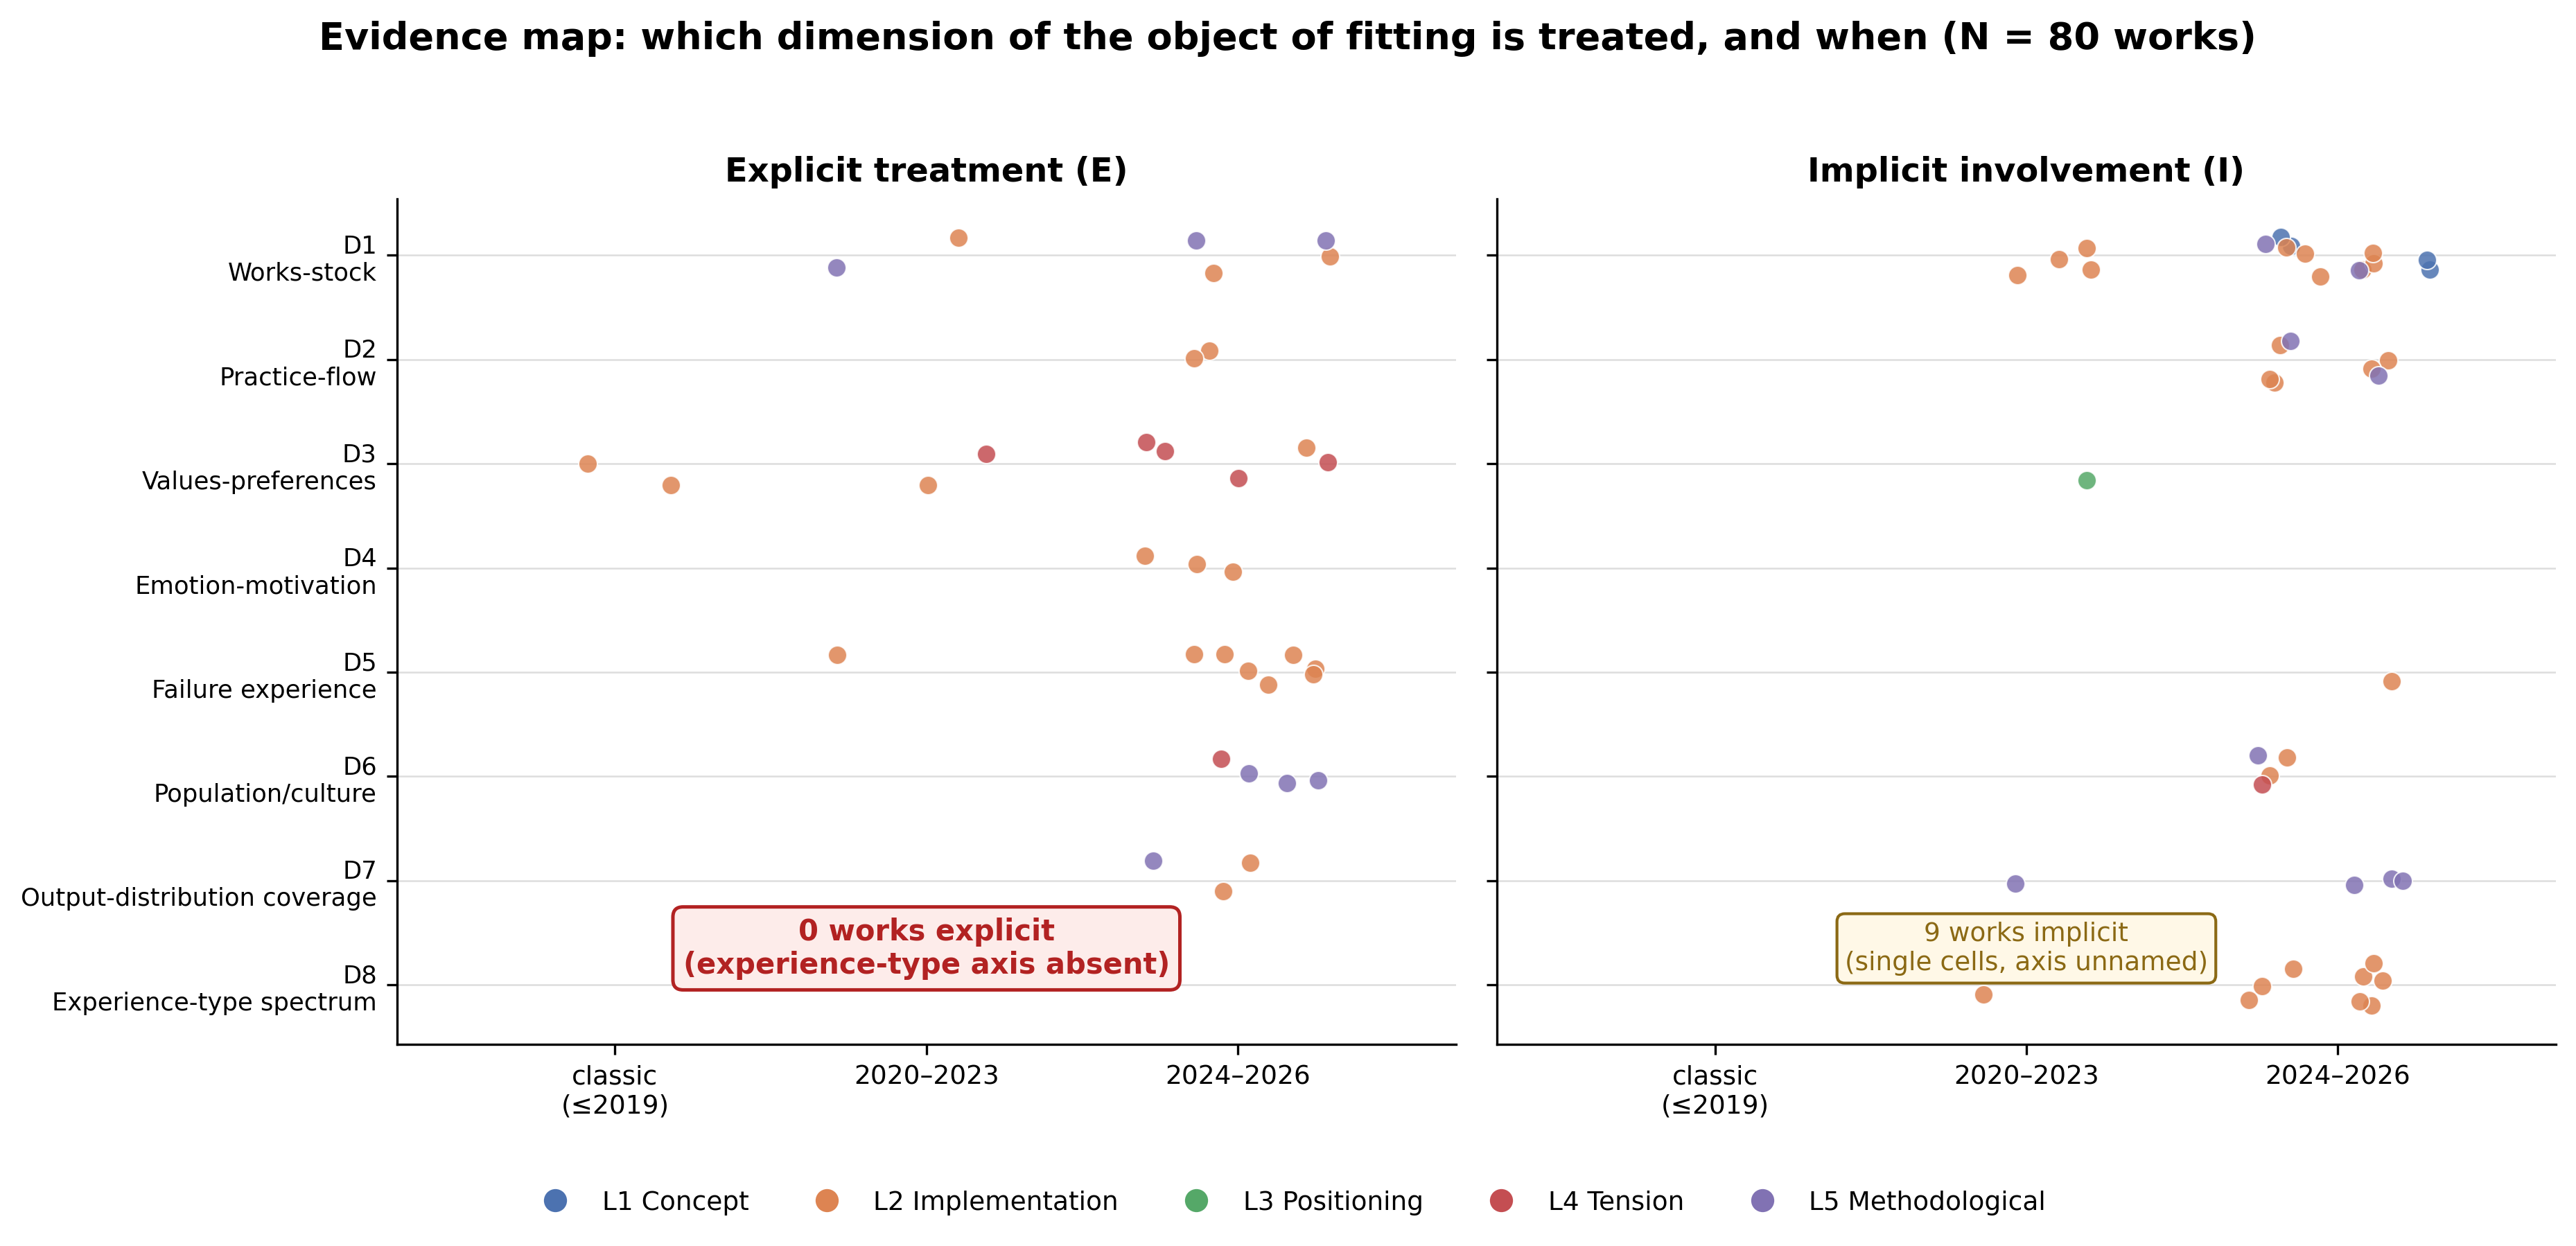
\includegraphics[width=\textwidth]{fig2_evidence_map.png}
\caption{80 篇语料的证据地图（年份分层 $\times$ 维度；点色 = 层级 L1--L5）。左板：显式处理（E）。右板：隐式涉及（I）。左板 D8 行为空——零篇作品，红框注释 “0 works explicit (95\% CI $[0, 4.5\%]$)”——而同一行在右板有九个隐式点（“single cells touched, axis never named”）。}
\label{fig:evidencemap}
\end{figure}

\begin{table}[t]
\centering
\caption{立场分布（A1 $\times$ A2，作品计数）。}
\label{tab:stance}
\begin{tabular}{lrrrrr}
\toprule
A1 $\backslash$ A2 & 增强 & 替代 & 反工具 & 未涉及 & 合计 \\
\midrule
支持       & 1 & 0 & 1 & 16 & \textbf{18} \\
否认       & 0 & 0 & 0 & 3  & \textbf{3} \\
未涉及     & 9 & 1 & 2 & 47 & \textbf{59} \\
\midrule
\textbf{合计} & \textbf{10} & \textbf{1} & \textbf{3} & \textbf{66} & \textbf{80} \\
\bottomrule
\end{tabular}
\end{table}

边际分布：A1 支持 18 / 否认 3 / 未涉及 59；A2 增强 10 / 替代 1 / 反工具 3 / 未涉及 66。地图的先验假设得到支持，外加一个有教益的细化：五份训练/系统技术报告全部为 A1-na（DeepSeek-V4.1 \cite{deepseek2026v41}、MiMo-V2.6 \cite{xiaomi2026mimo}、GLM-5 \cite{zai2026glm5}、Llama 3 \cite{grattafiori2024llama3}、DeepSeek-R1 \cite{deepseek2025r1}）——技术报告不讨论拟合，尽管官方\emph{实证}报告可以（可解释性发现 \cite{anthropic2026emotions} 为 A1-支持）；认知—实证作品集中于支持（4/5）；超人类成就研究路线否认（2/2，外加一个概念性否认 \cite{imeri2025benefits}）；坍塌/覆盖研究路线分裂：三篇作品全部显式处理输出分布（D7=E：蜂群研究 \cite{jiang2025hivemind}、模型坍塌 \cite{shumailov2024collapse}、Spectrum Tuning \cite{sorensen2025spectrum}），其中经验坍塌证据为 A1-支持 \cite{jiang2025hivemind}，动力学与方法学工作为 na \cite{shumailov2024collapse, sorensen2025spectrum}——覆盖研究路线不主张“拟合人类”，它测量分布后果。

解耦设计解决了预先料到的混合案例：图灵陷阱是 A1-支持 $\times$ A2-增强（记录路线级范围）；Vallor 是 A1-支持 $\times$ A2-反工具（批评的是拟合的\emph{质量}而非其发生）；蜂群研究是 A1-支持 $\times$ A2-na。Suleyman 的作品按文档分别编码（编码手册规则 CR2）：2023 年的书定位替代 \cite{suleyman2023coming}；2026 年 9 月的声明集定位增强 \cite{suleyman2026personable}。

\begin{figure}[t]
\centering
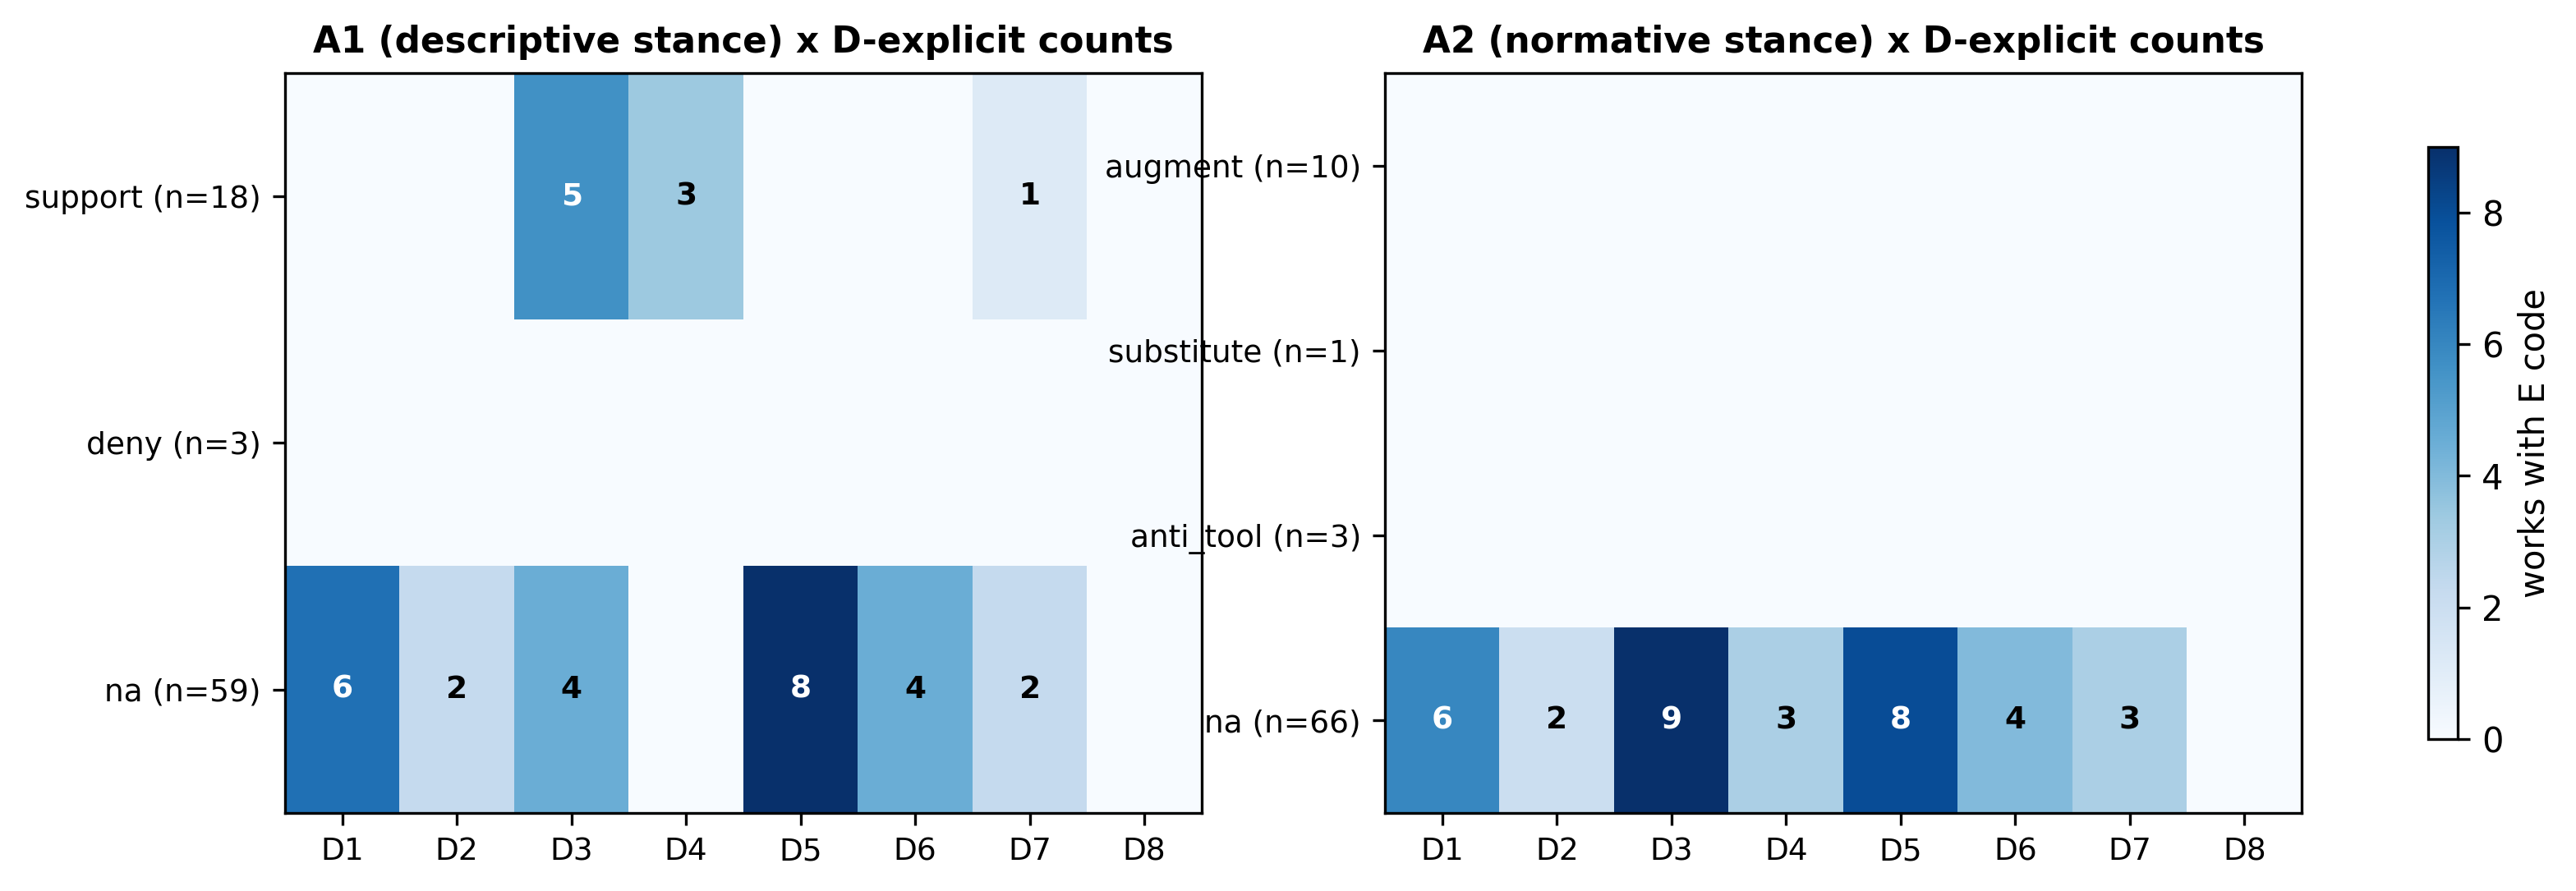
\includegraphics[width=\textwidth]{fig3_stance_dimension_heatmap.png}
\caption{立场 $\times$ 维度热图（显式 E 作品计数）。左：描述性立场 A1 $\times$ 维度。右：规范性立场 A2 $\times$ 维度。左图全零的\emph{否认}行与右图全零的\emph{替代}行把下述结构性发现可视化：框架级否认与主体替代主张不伴随任何维度层面的具体设计。}
\label{fig:heatmap}
\end{figure}

结构性发现值得单独一句：图~\ref{fig:heatmap} 左板的\emph{否认}行全空，右板的\emph{替代}行亦然。在描述意义上且限于本语料：三篇 A1-否认作品无一携带任何维度码（显式或隐式均 0/3），而 A1-支持作品中为 16/18——否认在框架层运作，不在设计层。（这些对比的探索性列联表连同 Fisher 精确检验在随仓库发布的分析报告中给出，未校正且不外推；我们刻意不在本文将其复述为推断性证据，因为目的性抽样不支持任何总体推断。）

\subsection{主要结果：一条未被命名的轴}\label{sec:unnamed}

\begin{table}[t]
\centering
\caption{拟合对象维度：显式（E）、隐式（I）、缺席（$\dminus$）处理的频次。}
\label{tab:dimensions}
\begin{tabular}{lrrrrr}
\toprule
维度 & E & I & $\dminus$ & \%E & \%E 或 I \\
\midrule
D1 作品存量                        & 6 & 16 & 58 & 7.5\%  & 27.5\% \\
\textbf{D2 实践流量}               & \textbf{2} & 7 & 71 & \textbf{2.5\%} & 11.2\% \\
D3 价值—偏好                       & 9 & 1  & 70 & 11.2\% & 12.5\% \\
D4 功能性情绪—动机                 & 3 & 0  & 77 & 3.8\%  & 3.8\% \\
D5 失败经验                         & 8 & 1  & 71 & 10.0\% & 11.2\% \\
D6 人群/文化（谁）                 & 4 & 4  & 72 & 5.0\%  & 10.0\% \\
D7 输出分布覆盖                    & 3 & 4  & 73 & 3.8\%  & 8.8\% \\
\textbf{D8 经验类型谱}             & \textbf{0} & \textbf{9} & 71 & \textbf{0.0\%} & \textbf{11.2\%} \\
\bottomrule
\end{tabular}
\end{table}

\textbf{D8-explicit $=$ 0/80（0.0\%）}，精确二项（Clopper--Pearson）95\% CI $[0.0\%, 4.5\%]$，三倍法则（rule of three）上界 $\approx 3.8\%$。该结果对置信度不敏感：剔除全部 8 篇低置信度作品后，D8-E $=$ 0/72，CI $[0.0\%, 5.0\%]$。与零同样重要的是对照模态：\textbf{D8-implicit $=$ 9/80}——失败数据工作（LEMA \cite{an2023lema}、PRM800K \cite{lightman2024verify}、SPAR \cite{spar2026f26}、ETO \cite{song2024trial}、UltraInteract \cite{yuan2024advancing}、DeepSeek-V4.1 \cite{deepseek2026v41}、MiMo \cite{xiaomi2026mimo}、GLM-5 \cite{zai2026glm5}）与蜂群研究 \cite{jiang2025hivemind} 各自只触及类型空间的\emph{单一格}（只有失败，或只有均值）；无一命名或操作化经验类型为覆盖轴。发现因此得以精确陈述：\textbf{话题被触及；轴从未被命名。} 这是理论第三覆盖轴主张的可计数形式。

\paragraph{缺席检索程序。}
零计数的力度，至多与其背后检索的力度相当。我们运行了预注册式缺席检索（8 个查询族，横跨 arXiv 全历史、ACL Anthology 域内检索与中文网络检索；日志见附录~\ref{sec:appendix-absence}）：全部命中按 D8-E 判据筛选（经验类型维度\emph{被命名为}覆盖/抽样轴，\emph{且}被用于设计数据、实验或指标）。零篇通过；八个近似命中族连同理由被记录。最接近命中的案例最有教益：智能体经验基准把“经验”当作智能体自身先前情节（属于时间维度，而非经验类型维度）；数据配比研究路线优化域权重；而最近的一对——两篇 2026 年工作把\emph{机器 rollout 中模型错误的多样性}塑造为探索/RL 信号 \cite{baek2026dfuser, liu2026leveraging}。后一对表明第三轴正从机器一侧被逼近，而人类数据一侧仍为零；我们的主张因此限定于“作为人类实践数据上的覆盖轴”，并将随着该轴被操作化而遭证伪。编码冻结之后，我们于 2026-10-19 对同一检索做了复核——复核锐化而非消解了这个零。\emph{文化与人群}的类型化覆盖如今已获产业级操作化：一个标注框架——跨预训练、微调、对齐与推理四个阶段测量文化信号的覆盖——与配套的 560 万样本标注语料 \cite{sahu2026culturefunnel}——按本文坐标，这是人群轴（D6），不是经验类型轴（D8）。\emph{轨迹}类型多样性已在 RL 后训练中以用户指定的类型分布被操作化 \cite{fu2026tjpo}——作用对象是模型自身的 rollout，仍是机器一侧。而“训练数据的多样性”已作为命名因子出现在 RLVR 的熵坍塌分析中 \cite{jin2025entropy}——指 RL 运行内的提示集多样性，不是人类实践语料的覆盖设计。三者的共同模式：与经验类型相邻的各轴正在获得操作化；人类实践上的经验类型轴仍是既未被命名也未被测量的那一条。图~\ref{fig:evidencemap} 展示合并结果：显式板中空缺的 D8 行，与右板实际的九个隐式点形成对照——轴被触及，从未被命名。

\subsection{时间模式}\label{sec:temporal}

\begin{table}[t]
\centering
\caption{按年份分层的显式处理（附 D8 隐式对照）。}
\label{tab:temporal}
\begin{tabular}{lrrrr}
\toprule
维度 $\times$ 模态 & $\leq$2019 & 2020--2023 & 2024--2026 & 合计 \\
\midrule
D1 显式       & 0 & 2 & 4 & 6 \\
D2 显式       & 0 & 0 & \textbf{2} & 2 \\
D7 显式       & 0 & 0 & 3 & 3 \\
\textbf{D8 显式} & \textbf{0} & \textbf{0} & \textbf{0} & \textbf{0} \\
D8 隐式       & 0 & 1 & 8 & 9 \\
\bottomrule
\end{tabular}
\end{table}

三行对照叙述了理论本身。作品即存量是\emph{成熟}纲领：D1-E 作品 2022--2026 连续出现（数据墙分析 \cite{villalobos2022data}、配比优化 \cite{xie2023doremi, ye2024data}、旗舰语料设计 \cite{grattafiori2024llama3, penedo2024fineweb}）。输出分布覆盖是\emph{正在形成}的自觉：D7-E 首现于 2024 年 \cite{shumailov2024collapse} 并获巩固 \cite{jiang2025hivemind, sorensen2025spectrum}。经验类型轴是\emph{缺失}的第三轴：每个分层均为 0。实践即流量是\emph{新芽而非建制}：D2-E $=$ 2/80，均来自 2026 年——DeepSeek 的员工提交失败案例的数据流（“we collect negative feedback and model failure cases submitted by internal employees at scale” \cite{deepseek2026v41}）与同期存量/流量工程文章 \cite{gharbi2026model}。我们特意如此措辞：两篇作品构成的是一个开端，而非一个趋势。

来自地图的两点限定。其一，WEIRD 悖论单元 \cite{zhou2025should}：提高训练数据的文化代表性可能\emph{放大}歧视性观点的复现——提高“谁”被代表，并不能修复“什么”被覆盖。覆盖问题因此是“两轴已知而未解”，不是“两轴已解”——这正是第三轴进入的空间。其二，一个探索性结构观察（描述性，仅限语料内）：显式的维度级设计集中于 A1-na 作品（至少有一个显式维度者 23 篇，A1-支持作品中为 9 篇）。结合第~\ref{sec:stance} 节的空否认行，模式是解耦：辩论 AI 是否拟合人类的人大多不做覆盖工程，做覆盖工程的人大多不辩论它。这一解耦是第~\ref{sec:intro} 节所述缺口——缺失的连接命题——在数据上的定量印证。

\subsection{证据地图的局限}\label{sec:maplimits}

持怀疑态度的审稿人也应当能够接受这些限度。(i) \textbf{无总体推断}：语料为按配额分层的目的性抽样；一切断言都是“本语料内”。(ii) \textbf{单一编码者}：$\kappa$ 重编码已排期（2026-10-29），目前尚不可得；缓解措施是公开的编码手册、强制的引文锚点与公开的边界案例日志。(iii) \textbf{严格饱和未达}：语料填满至 80 篇上限并报告缺口。(iv) \textbf{缺席断言受程序约束}：0/80 的零计数，加上八个查询族的缺席检索，在其窗口内（2026-10-15 关闭）是有力的，但并非永远成立。(v) \textbf{核心断言与置信度无关}（第~\ref{sec:unnamed} 节敏感性分析），但 8 个单元仍为低置信度、留待核验。(vi) 地图约束的是\emph{描述性}断言；第~\ref{sec:position} 节的\emph{规范性}立场是论证的选择，不是地图结果。

\subsection{同期工作与整合划界}\label{sec:concurrent}

两篇同期工作被标记并划界（隔离优先权断言是一项诚实要求，不是形式主义）。\textbf{Gharbi 的 SSRN 文章} \cite{gharbi2026model} 以显式的存量/流量工程框架分析数据墙的九条逃生路线，并识别出数据墙之后的“验证者墙”——与我们的时间性条款最接近的已发表表述。划界是锐利的：它是数据工程。它不含作品与实践的本体区分，没有全谱 $\times$ 全程坐标系，没有覆盖轴，没有工具定位；它的流量是供应链，不是拟合对象。其 D1-E/D2-E 编码在专门的补充材料（表~\ref{tab:gharbi}）中单独报告，不计入理论的缺口断言。\textbf{Fenoglio 的非对称交流文章} \cite{fenoglio2026asymmetric} 论证 LLM 输出在承诺不对称之下于人类实践中获得意义——一个关于意义的理论，没有拟合纲领、没有增强定位、没有坐标系。第三篇同期工作从经济学抵达同一存量/流量结论：一个人类数据市场理论把结构化人类数据工作——评估、量表判断、审计、异常处理——建模为持续的劳动\emph{流}，累积为折旧的能力存量 \cite{ansari2026nolastmile}；它处理的是流的市场，不是流的拟合，且不提供覆盖轴与训练数据设计。跨学科汇聚而无重叠。三篇同期工作都未主张时间性条款的三要素组合（实践而非作品 + 全谱 $\times$ 全程 + 存量有墙/流量无墙）；截至窗口关闭，该组合的优先权仍归本文。

\begin{table}[t]
\centering
\caption{本理论与相邻框架。}
\label{tab:frameworks}
\small
\begin{tabular}{p{0.26\textwidth}p{0.32\textwidth}p{0.34\textwidth}}
\toprule
框架 & 提供 & 缺失（本理论所补） \\
\midrule
文化技术 \cite{farrell2025cultural, yiu2024transmission} & 描述性分类：LLM 继承人类符号结构 & 时间性区分（作品与实践）；覆盖轴；数据方法论后果 \\
\addlinespace
批判现象学（镜子） \cite{vallor2024mirror} & 警告：扭曲的反射重塑人类自我理解 & 忠实拟合的建设性说明；全谱/全程坐标；边界条件 \\
\addlinespace
增强经济学 \cite{brynjolfsson2022turing, engelbart1962augmenting, shneiderman2022human} & 规范目标：互补优先于替代；设计点（控制 $\times$ 自动化） & 拟合本体论（为何模仿作为\emph{手段}不同于作为\emph{目的}）；终止边界 \\
\addlinespace
存量/流量数据工程 \cite{gharbi2026model}（同期） & 供给侧分析：逃生路线、验证者墙 & 实践本体论；第三覆盖轴；工具定位 \\
\bottomrule
\end{tabular}
\end{table}

\section{张力与边界}\label{sec:tensions}

理论最后处理第四个层面：拟合在哪里自我绷紧，又在哪里停止。

\paragraph{价值多元主义：谁的谱？}
全谱在是“什么”问题之前先是“谁”问题。对齐文献早已认识到，价值拟合未定谁的价值 \cite{gabriel2020values}；多元对齐路线图把多元性跨人群操作化 \cite{sorensen2024roadmap}；社会选择批判表明，偏好聚合预设了存在争议的规范承诺（对异质反馈的功利主义与词典式最小化（leximin）聚合） \cite{park2024rlhf}；聚合问题分析编目其失败模式 \cite{baum2025aggregation}；约 1,000 名（美国）参与者的集体宪法实验同时证明了当下集体过程的可行性与\emph{地理窄化} \cite{huang2024collective}。谱轴不消解这一张力——它继承之。全谱拟合仍需一个聚合决定，这正是第~\ref{sec:implications} 节将治理单列一问的原因。

\paragraph{主体性边界：永不人格化，永不拟合现象状态。}
语料中最尖锐的现实冲突富有教益。Anthropic 的模型福祉计划追问模型是否可能值得道德考量 \cite{anthropic2025welfare}；Suleyman 2026 年 9 月的言论公开拒绝该路线：AI 应是可亲的（personable）工具——有个性——但绝不授予人格地位 \cite{suleyman2026personable}。我们把此读作对立阵营之间的一次意外结盟，并基于独立理由持有该立场：永不授予人格地位与永不拟合现象状态，是同一条边界的两面。拟合目标包括功能性情绪—动机结构——而因果功能性情绪概念的可解释性证据 \cite{anthropic2026emotions} 确认这一层\emph{正在}被拟合——但理论的边界恰好落在功能层：对感受经验，理论不作断言——既不肯定，不许可，亦无此需要。镜子批判 \cite{vallor2024mirror} 提供互补的警告：被拟合之镜的危险不在于它感受，而在于它的反射重构人类对自身的理解。

\paragraph{中国脉络：一条没有主体性语言的平行线。}
官方中国 AI 治理谱系从 2019 年治理原则（负责任 AI 的“以人为本”发展） \cite{govcn2019principles}，经 2023 年全球人工智能治理倡议 \cite{govcn2023initiative}，到 2025 年国务院“人工智能+”行动意见 \cite{govcn2025aiplus}——一部这样的政策文本语料：充满\emph{赋能}与\emph{人机协同}的词汇，而不含主体性归因。古典根源以罕见的简洁契合工具立场：庄子的“物物而不物于物” \cite{zhuangzi2016complete} 在工具范畴辩论之前二十三个世纪就陈述了掌握条件——使用工具，而不被工具使用。在我们的语料内，儒家角色伦理单元可读作对朴素纯工具解读的一次内部矫正（护理机器人无法履行孝式义务），记录于地图注记而不作过度解读。

\paragraph{四条终止边界。}
时间性条款止于其术语止步之处；理论显式划定四条边界。
\begin{itemize}
\item \textbf{B1——实践主体的终结。} 流量随生命再生；最后一次实践之后，拟合无对象。（一条生存性边界，不是工程边界。）
\item \textbf{B2——拟合者越界。} 若拟合者超越每一位教师——称之为 ASI——拟合关系便自行耗尽：已不存在不落在它身后的人类实践可供拟合。本理论的对象是以人为参照的 AGI 概念；越过此边界，理论刻意沉默，仅作标记。
\item \textbf{B3——制度边界。} 法律、隐私与知情同意约束可采集之物；第~\ref{sec:position} 节的规范性立场还反向定义了对流量的取用权——工具立场不仅约束 AI 为何而造，也约束它可以取走什么。（上文多元主义张力即处于此边界之内。）
\item \textbf{B4——自指性污染。} 一旦 AGI 织入日常，被采集的实践已被 AGI 染色：拟合目标被拟合这一行为本身改变——镜子进入了它所反射的房间。这是模型坍塌在流量体制下的新形态 \cite{shumailov2024collapse}：不是静态存量上的递归，而是活流的污染。缓解是工程而非禁止：原生与 AI 中介实践的出处分层标注（留待未来工作的协议组件）。
\end{itemize}

\paragraph{可证伪性。}
理论点名自己的证伪者。若流量侧被证明有一堵与存量墙同构的硬墙（例如一个击败持续学习的原则性下界），或若全谱拟合可证地在任意尺度坍塌为均值，时间性条款便弱化为一个启发式。若显式的经验类型覆盖在中性文献中频繁出现，第三轴缺口断言（0/80）失败——2026 年到来的相邻操作化（人群轴的文化覆盖 \cite{sahu2026culturefunnel}；轨迹类型多样性 \cite{fu2026tjpo}；RL 提示集多样性 \cite{jin2025entropy}）尚不构成那次失败，其区分在结果陈述处（第~\ref{sec:unnamed} 节）给出。若实践流数据被证明无法以生产级质量建造，D2-E 计数（2/80）作为证据失败。这些被陈述出来，是为了让理论可以输。

\section{方法论蕴含}\label{sec:implications}

从理论到方法：对下面三个问题中的每一个，我们陈述问题、证据地图所显示的现状、以及答案的形态。完整协议留待未来工作。

\paragraph{分布 $=$ 全谱覆盖。}
在当前实践中，多样性目前以三种角色出现：作为回归变量（域权重优化 \cite{xie2023doremi, ye2024data}，及隐式多语言配额如 Llama 3 的 8\% \cite{grattafiori2024llama3}）；作为局部启发式（十亿规模的人物设定（persona）条件化合成 \cite{ge2024scaling}）；以及作为质量过滤的牺牲品（教育语料策展按约 92\% 的比例弃置原始网络 \cite{penedo2024fineweb}）。把覆盖作为显式后训练目标的转向——针对指令微调坍塌恢复分布覆盖 \cite{sorensen2025spectrum}——是朝正确方向迈出的一步，但它覆盖的是\emph{输出分布}轴；人群轴有自己的研究路线（多语言策展，如 65 语言指令集合 \cite{singh2024aya}；文化信号覆盖如今已获产业级标注 \cite{sahu2026culturefunnel}）；经验类型轴则为 0/80（第~\ref{sec:unnamed} 节）。WEIRD 悖论 \cite{zhou2025should} 警告，朴素的人群配额会反噬（代表“谁” $\neq$ 修复“什么”被覆盖），因此全谱覆盖必须整合各轴而非堆叠配额。我们刻意用“覆盖”，不用“配额”。

\paragraph{生产 $=$ 永续采集协议。}
流量侧需要一套组织机制，其先例可见：规模化的员工提交失败案例 \cite{deepseek2026v41}；智能体训练中的失败反思与错误保留实践 \cite{xiaomi2026mimo, zai2026glm5}；以及迄今最宽的制度级先例——消费者条款把进行中的对话与编码会话导入训练（附可退出条款） \cite{anthropic2025consumerterms}，一个直接接入实践流而非作品存量的入口。协议组件在此定义、待未来工作细化：把失败案例当作与成功数据同等地位数据的采集协议；以区分真失败与奖励作弊式伪失败为要点的毒性数据清洗（审计论文的边界条件 \cite{yu2026failure}）；三段式记录结构（错误类型、根因、纠正）；以及针对任何合成增强的坍塌防护——如今有了量化的锚：指数族中每步单个真实数据点即可证明性地阻止闭环坍塌 \cite{jangjoo2026lost}，污染下的收敛由真实数据占比支配 \cite{wang2026guarantees}，累积式训练能保住替换式训练所毁掉的（该机制已由先于模型坍塌出现的“筛选坍塌”独立复证 \cite{zhang2026screening}），且退化是不对称的——已强的技能被强化而已弱的技能继续衰减 \cite{luo2026polarization}——因此掺混下限必须按能力类型分别设定，而非全局设定。约束瓶颈不是采集而是\emph{吸收}：实践每日再生而模型快照按周期更新——\emph{拟合时差}——且智能体的稳定性—可塑性两难仍未解决 \cite{wu2026agentdice}。尽管如此，吸收正在变得可行：时间增量持续预训练在开源权重规模上被证明无灾难性遗忘 \cite{oncel2026timeincremental}，自生成回放近乎消除参数记忆的遗忘 \cite{marek2026replay}——这使“未披露分层时差指标”成为透明的瓶颈，而非研究未知。地图把吸收侧工作编码为 D2-隐式：其数据源（尚）未被规定为实践流。（证据窗口关闭后，报道显示前沿实验室如今并行运行数以万计的 RL 训练演练，由模型配置、监控与评分 \cite{nolan2026fortune}——规模化故事的重心正从数据存量移向 RL 过程，而这正是流问题落地之处。）

\paragraph{治理 $=$ 多元聚合与制度。}
谁聚合谱、谁许可流、谁裁定失败：聚合工具箱横跨社会选择机制 \cite{park2024rlhf}、多宪法过程 \cite{huang2024collective}、人物设定条件化生成 \cite{ge2024scaling} 与主权本地模型；许可权直面出处权利在少数大出版商手中的集中；而验证者问题——谁认证一个失败是失败——是整个飞轮转动所依的轴承 \cite{yu2026failure, gharbi2026model}。B4 的缓解（原生与 AI 中介出处分层）同样是对数据基础设施的一项制度要求，而不仅仅是一种标注约定——而且它正在变成工程可行项：经签名过滤增强的统计水印检测，在低熵信号强度下已能达到 78--99\% 的准确率 \cite{hong2026signature}。

\section{结论}\label{sec:conclusion}

本文论证了一个三层论题：AGI 是一个以人类实践为参照系的哲学概念；其实现是对该实践的拟合——作品即存量是静态误读的成熟形态，实践即流量是正确解读的开端；其恰当位置是增强性工具，一个必须由制度持续防御的规范性选择。证据地图使理论的主张可计数：一个 80 篇作品的语料，其中经验类型覆盖轴从未被命名（0/80；95\% CI $[0.0\%, 4.5\%]$），实践即流量仅在两篇作品中显式（均 2026 年），且立场与对象在文献中解耦——描述性、规范性与方法论文献各自成熟，未被那个需要三者兼备的命题所连接。理论的贡献就是那个命题、它的坐标系、它的边界与它点名的证伪者。

本文在理论开始之处收束。下面这句话区分了本领域的两种未来——积累档案直至高墙，或拟合再生中的实践：

\begin{quote}
\textbf{拟合对象不是人类的作品，而是人类的实践——人类经验的全谱（横截面）与全程（纵截面）。存量有墙，流量无墙。}
\end{quote}

流量是否被拟合好——跨全谱、沿全程、在四条边界之下、朝向增强——不是一个等待应验的预测，而是一个有待执行的纲领。其执行留待未来工作。

\medskip
\paragraph{数据与代码可用性。}
语料（corpus\_v1，80 篇作品 $\times$ 24 个变量）、编码手册、缺席检索日志、全部表格 CSV、图（300 dpi）与单文件复现脚本（\texttt{analysis/coding\_data.py}；seed 20261015）随论文仓库发布。配套审计论文的完整材料：DOI 10.5281/zenodo.23355929。

\paragraph{AI 辅助披露。}
沿用配套审计论文的做法：文献检索、核验、编码与起草在作者监督与规则化协议（编码手册规则 R1--R5、CR1--CR6；核验日志见随仓库发布的分析报告）之下借助 AI 完成；全部编码断言附逐字或设计锚点，单一编码者的局限在第~\ref{sec:maplimits} 节披露。

\paragraph{利益冲突。}
无声明。本研究在独立研究机构（余玉桂战略研究室）完成，无外部资助，与其公开文件被分析的组织无财务关系。

\appendix

\section{缺席检索日志（2026-10-14 执行）}\label{sec:appendix-absence}

支撑 D8-explicit $=$ 0/80 断言（第~\ref{sec:unnamed} 节）的预注册式缺席检索：三个引擎（arXiv 全历史；ACL Anthology 域内检索；中文网络检索）上的八个查询族。筛选判据（两个合取项均需满足）：(i) 经验类型维度（成功/失败 $\times$ 专家/新手 $\times$ 典型/边缘）被命名为覆盖/抽样/分层轴；(ii) 该轴被用于设计数据、实验或指标。结果：\textbf{0 篇通过；八个近似命中族连同理由被记录}。代表性命中附可核验的标识符；包含全部命中的完整日志随仓库发布。编码冻结后于 2026-10-19 执行的同一检索复核（与它所重检的结果一并报告于第~\ref{sec:unnamed} 节）再次返回 0 篇通过；复核所浮现的最近邻命中，其划界见该节。

\begin{table}[h]
\centering
\caption{缺席检索日志：八个查询族，0 个 D8-E 命中。}
\label{tab:absence}
\footnotesize
\begin{tabular}{p{0.05\textwidth}p{0.30\textwidth}p{0.55\textwidth}}
\toprule
\# & 查询族（引擎） & 代表性命中与注册的近似命中理由 \\
\midrule
Q1 & “success and failure” coverage training（arXiv） & 持续预训练合并（2511.02451）；用户编辑微调（NeurIPS 2025）。定性案例分析，无覆盖轴设计。 \\
Q2 & “expert” “novice” data mixture（arXiv） & SimInstruct（2508.04428）把专家—新手对话生成为\emph{数据类型}，而非配比/覆盖轴；配比研究路线（2502.15950、2607.01104、2601.17858）优化域权重。 \\
Q3 & “experience type” coverage（arXiv） & AhaBench（智能体从先前情节学习）；VCR（AAAI 2025）。“经验”= 智能体自身情节（时间性），非类型谱——最接近命中的案例，逐条记录。 \\
Q4 & “error diversity” curriculum（arXiv） & DiVERT（2406.19356，EMNLP 2024）；GEC 数据加权。错误多样性用于干扰项生成/纠错，非拟合数据覆盖。 \\
Q5 & “typical” “edge” spectrum coverage（arXiv） & 自动驾驶边缘案例综述（2410.08491）；角落案例生成。典型到边缘的谱系被操作化为场景测试，非人类实践拟合数据。 \\
Q6 & 中文网络：成功/失败案例比例；专家/新手覆盖 & LLM 训练数据综述（2411.07715）；数据瓶颈的新闻报道。唯一在命题层面接近命中的是一篇媒体报道（T3 可信度层，非一手来源；仅动机层提及，按一手来源规则排除）。 \\
Q7 & success failure expert novice coverage data selection（ACL Anthology） & 数据选择研究路线（Albalak 2402.16827；ACL 2025；LESS）。以影响力/质量为轴；无经验类型轴。 \\
Q8 & “error diversity” / “failure diversity” training coverage（arXiv） & \textbf{D-FUSEr}（ICML 2026，PMLR 306）；\textbf{EDAS}（2605.17333）。两者都塑造\emph{模型 rollout} 的错误分布（机器一侧多样性作为探索/RL 信号），非人类经验类型覆盖——最重要的一对近似命中：第三轴正从机器一侧被逼近，而人类数据一侧仍为零。 \\
\bottomrule
\end{tabular}
\end{table}

\section{补充材料 S1：同期工作编码行（Gharbi）}\label{sec:appendix-gharbi}

\begin{table}[h]
\centering
\caption{补充材料 S1：同期存量/流量数据工程文章（按同期工作规则处理）的单独报告的编码记录，单独报告，不计入理论的缺口断言（第~\ref{sec:concurrent} 节）。}
\label{tab:gharbi}
\small
\begin{tabular}{p{0.16\textwidth}p{0.72\textwidth}}
\toprule
作品 & W-038：Gharbi（2026），SSRN 预印本 7479298（2026-09-17） \\
\midrule
编码 & A1 = na；A2 = na；D1 = E；D2 = E；D2-explicit = True；concurrent = True；置信度 = 中 \\
划界 & 工程意义的存量/流量 $\neq$ 实践本体论：无作品与实践之分、无全谱 $\times$ 全程框架、无覆盖轴、无工具定位 \\
\bottomrule
\end{tabular}
\end{table}

\bibliographystyle{unsrtnat}
\bibliography{references_zh}

\end{document}
